\documentclass{article}
\usepackage{amsmath}
\usepackage{physics}
\usepackage{graphicx}
\usepackage{mathrsfs}
\usepackage{amssymb}
\usepackage{microtype}
\usepackage{listings}
\usepackage{xcolor}
 
\definecolor{codegreen}{rgb}{0,0.6,0}
\definecolor{codegray}{rgb}{0.5,0.5,0.5}
\definecolor{codepurple}{rgb}{0.58,0,0.82}
\definecolor{backcolour}{rgb}{0.95,0.95,0.92}
 
\lstdefinestyle{mystyle}{
    backgroundcolor=\color{backcolour},   
    commentstyle=\color{codegreen},
    keywordstyle=\color{magenta},
    numberstyle=\tiny\color{codegray},
    stringstyle=\color{codepurple},
    basicstyle=\ttfamily\footnotesize,
    breakatwhitespace=false,         
    breaklines=true,                 
    captionpos=b,                    
    keepspaces=true,                 
    numbers=left,                    
    numbersep=5pt,                  
    showspaces=false,                
    showstringspaces=false,
    showtabs=false,                  
    tabsize=2
}
 
\lstset{style=mystyle}

\newcommand{\RN}[1]{%
  \textup{\uppercase\expandafter{\romannumeral#1}}%
}
\title{Appendix}
\begin{document}
\author{Ha Nul Seok}
\maketitle
\section*{A. Deriving Maxwell's curl equation}
Maxwell's curl Eqaution is:
\begin{equation}
    \nabla \times E = - \frac{\partial H}{\partial t}
\end{equation}
\begin{equation}
    \nabla \times H =  \frac{\partial E}{\partial t}
\end{equation}
Solve the Del operation in the LHS for 1D case(propagates to y direction only),
\begin{equation}
    \nabla \times E = \det\begin{vmatrix}
                            \hat{i} & \hat{j} & \hat{k} \\
                            \frac{\partial}{\partial x} & \frac{\partial}{\partial y} & \frac{\partial}{\partial z} \\
                            E_x & 0 & 0
    \end{vmatrix}
    =\partial_y E_x = \frac{E_x(z+\Delta z,t)-E_x(z,t)}{\Delta z}
\end{equation}
\begin{equation}
    \nabla \times H = \det\begin{vmatrix}
                            \hat{i} & \hat{j} & \hat{k} \\
                            \frac{\partial}{\partial x}s & \frac{\partial}{\partial y} & \frac{\partial}{\partial z} \\
                            0 & 0 & B_z
    \end{vmatrix}
    = -\partial_x H_z = \frac{H_z(x+\Delta x,t)-H_z(x,t)}{\Delta x}
\end{equation}
Since E, B is function of $r,t$, RHS of the given Equation are:
\begin{equation}
    - \frac{\partial H}{\partial t} = \frac{H_z(x+\Delta x , t + \Delta t)-H_z{x+\Delta x, t}}{\Delta t}
\end{equation}
\begin{equation}
    \frac{\partial E}{\partial t} = \frac{E_x(z+\Delta z , t + \Delta t)-E_x(z+\Delta z, t)}{\Delta t}
\end{equation}
Substitute on Eq.(1),(2),
\begin{equation}
    -\frac{E_x(z+\Delta z,t)-E_x(z,t)}{\Delta x} =  -\frac{H_z(x+\Delta x , t + \Delta t)-H_z(x+\Delta x, t)}{\Delta t}
\end{equation}
\begin{equation}
    \frac{H_z(x+\Delta x,t)-H_z(x,t)}{\Delta y} =  \frac{E_x(z+\Delta z , t + \Delta t)-E_x(z+\Delta z, t)}{\Delta t}
\end{equation}
Finally,
\begin{equation}
    \frac{E_x(z+\Delta z,t)-E_x(z,t)}{\Delta x} - \frac{H_z(x+\Delta x, t)}{\Delta t} =  \frac{H_z(x+\Delta x , t + \Delta t)}{\Delta t}
\end{equation}
\begin{equation}
    \frac{H_z(x+\Delta x,t)-H_z(x,t)}{\Delta x} + \frac{E_x(z+\Delta z, t)}{\Delta t}  = \frac{E_x(z+\Delta z , t + \Delta t)}{\Delta t}
\end{equation}
\section*{B.Trial to Get the Energy band}
\begin{figure}[h]
    \centerline{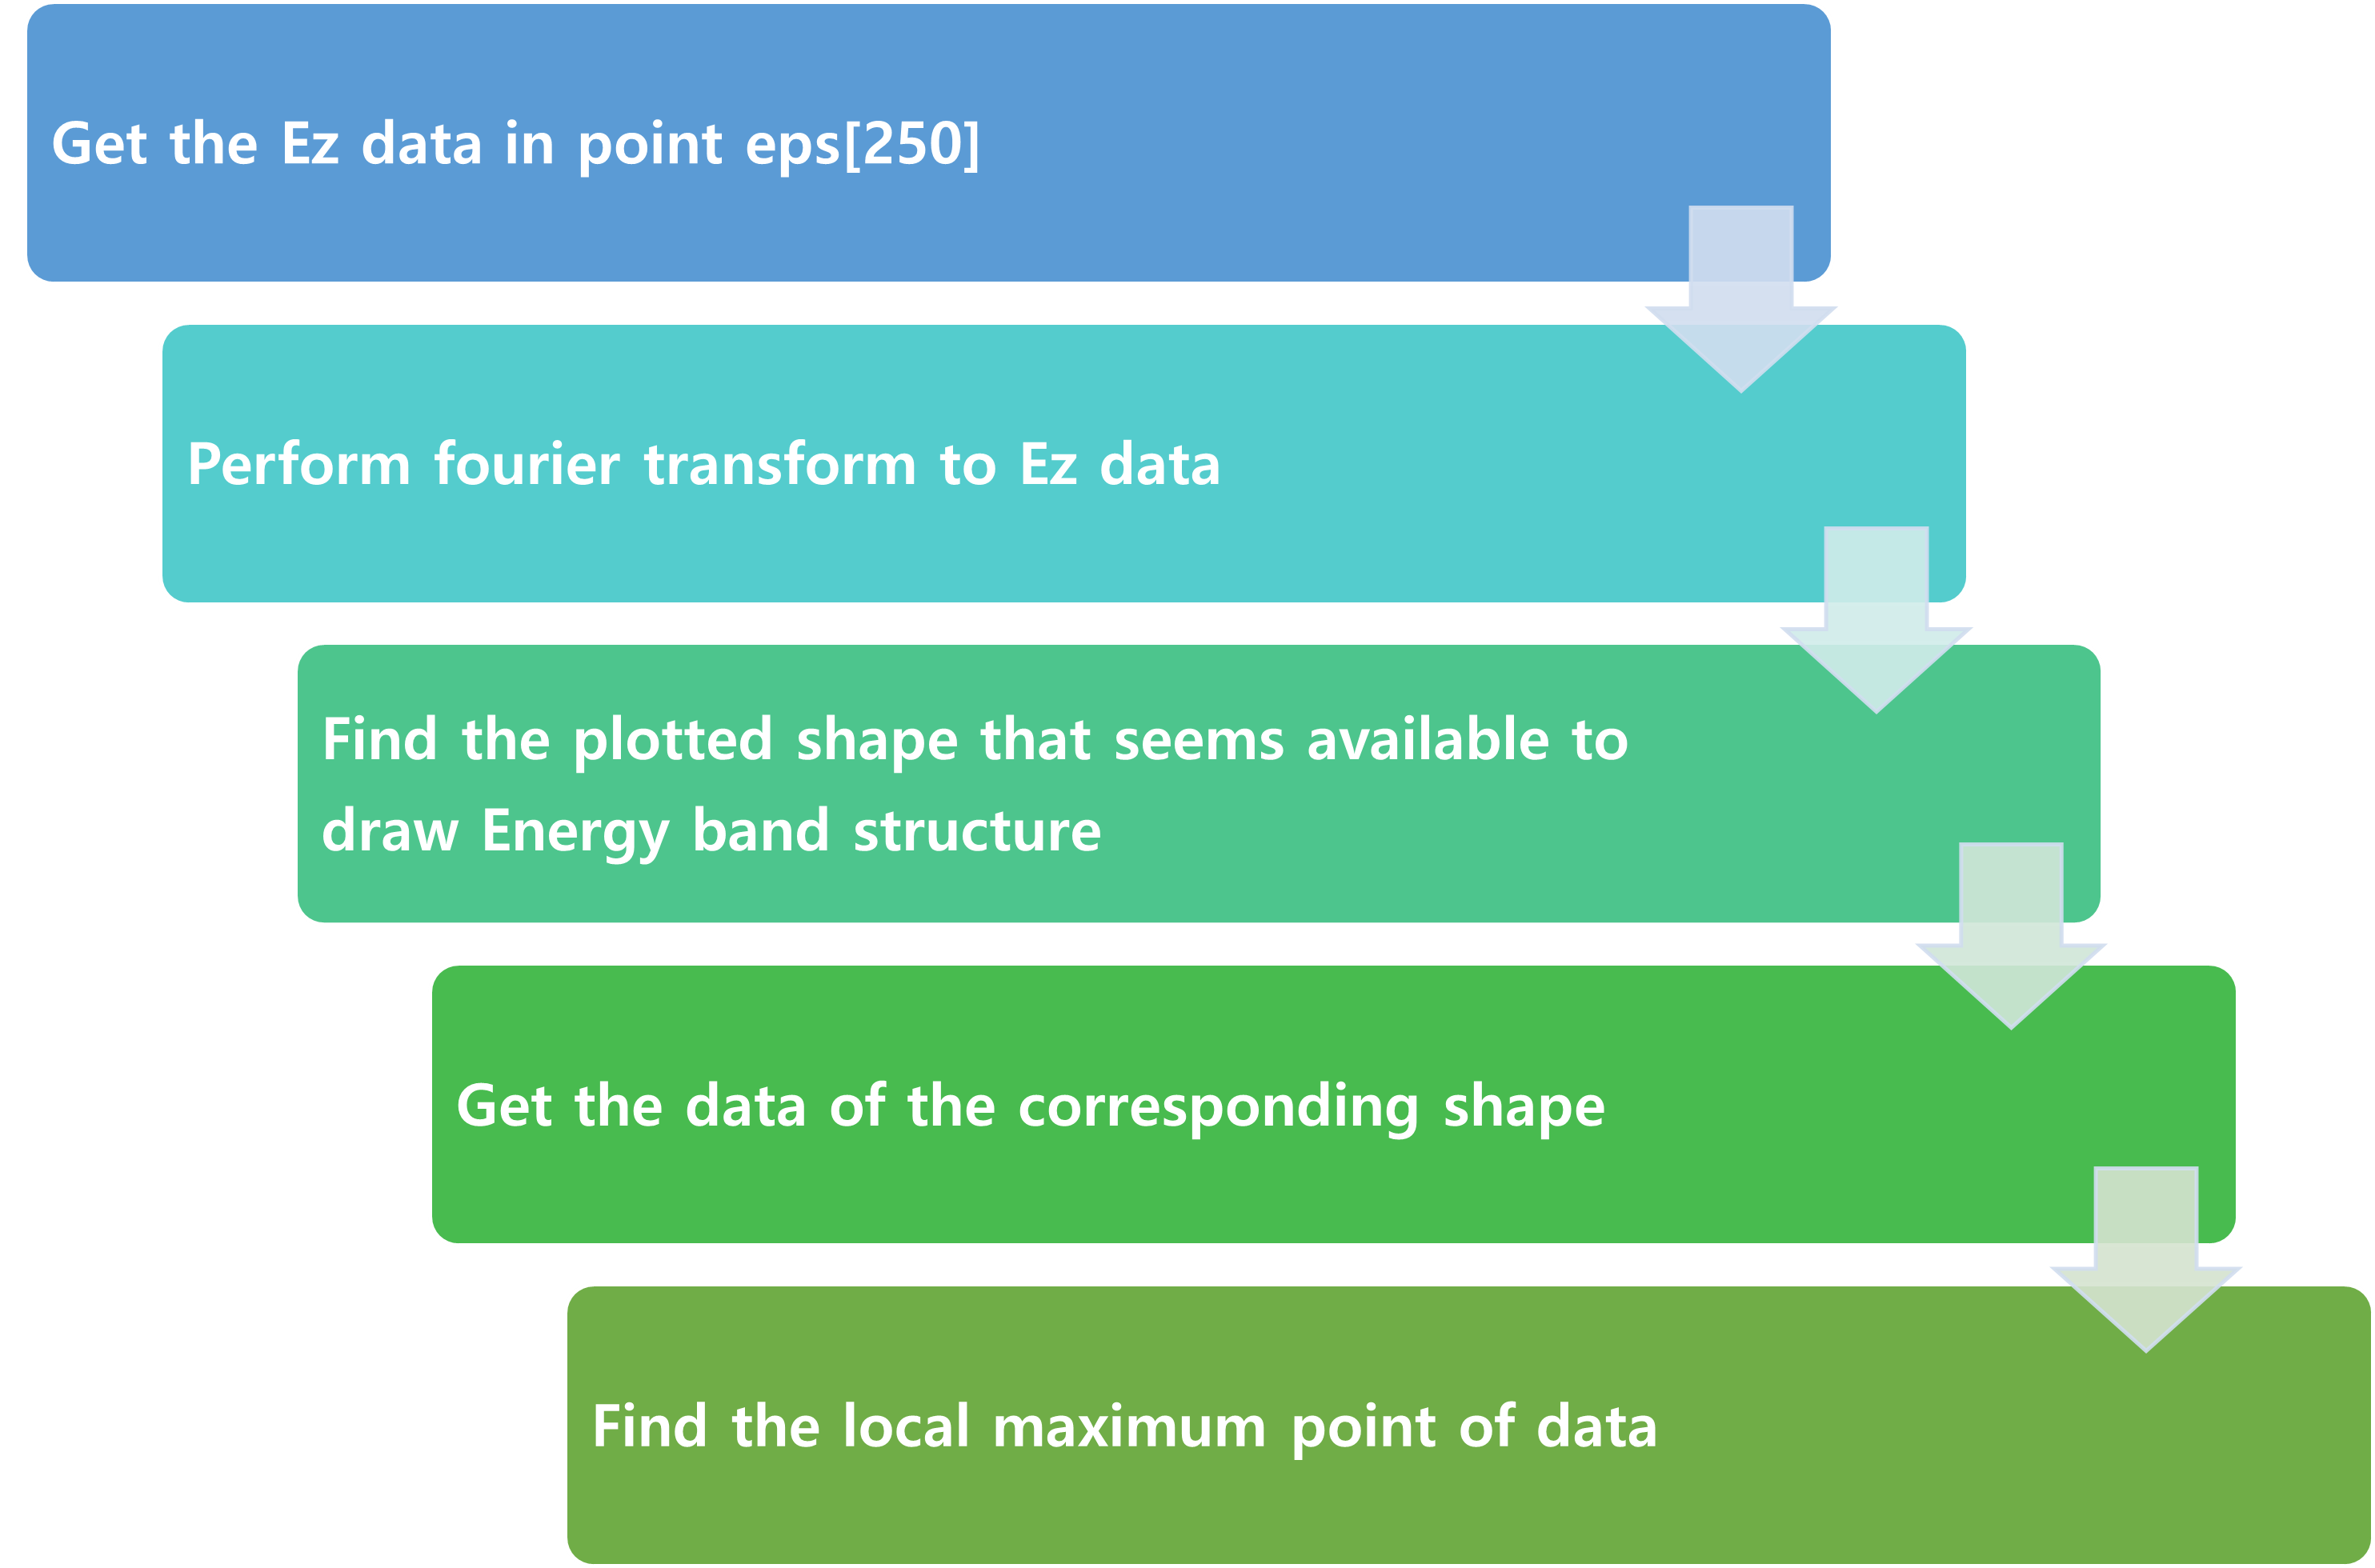
\includegraphics[width=\columnwidth]{20230618.png}}
    \caption{Steps to Draw a Band}
    \label{figure_1} 
\end{figure}
Trial to draw a Energy band can seperated into 5 steps. First, Get the Ez data from the spatial point
corresponds with eps[250]. Next, Perform fourier transform to Ez data. the result plot follows in Figure 2.\\ \\
 There are two peaks, one is in negative domain and one is in positive domain. We choose the peak shape in positive domain to Get the data, showed in Figure 3.
Reason that neglects the negative side is that, we must consider imaginary part of frequency if we consider the negative frequency.
\\
\\
In Fourth step, to get the maximum point of frequency plot, following codes are used:
\begin{lstlisting}[language=Python, caption=Fourier data and for loop to get local maximum.]
fourier_points = [0.00137213, 0.00169687, 0.00119211, 0.00104168, 0.0029928 ,
        0.00247675, 0.00184276, 0.00186229, 0.00129526, 0.00180773,
        0.00443303, 0.00238777, 0.00146412, 0.00143457, 0.00229274,
        0.00425652, 0.0037831 , 0.00251019, 0.00470327, 0.00439227,
        0.00497154, 0.0063496 , 0.00439958, 0.00235421, 0.00483729,
        0.00393799, 0.00104501, 0.00132122, 0.00242898, 0.00464641,
        0.01100574, 0.00628542, 0.00440889, 0.00216396, 0.00519568,
        0.00981485, 0.0079608 , 0.00261002, 0.00673896, 0.00484558,
        0.00132809, 0.00317639, 0.00530858, 0.01191112, 0.01227691,
        0.00583243, 0.00238056, 0.00669509, 0.00750436, 0.0067248 ,
        0.00176626, 0.00338634, 0.00779347, 0.00415383, 0.00565098,
        0.00676187, 0.00935157, 0.01001974, 0.00307908, 0.00799344,
        0.00725298, 0.0067394 , 0.00271255, 0.00179979, 0.00246135,
        0.00530239, 0.00475961, 0.00304775, 0.00436681, 0.0067991 ,
        0.00951265, 0.00601259, 0.00286832, 0.00227501, 0.00312039,
        0.00374843, 0.00111174, 0.00207669, 0.00619195, 0.00309905,
        0.00228059, 0.00239001, 0.00348588, 0.00660836, 0.00267389,
        0.00138811, 0.00137993, 0.00225289, 0.0028209 , 0.00218393,
        0.0019114 , 0.00201147, 0.00193926, 0.00136766, 0.00107451,
        0.00132982, 0.00106145, 0.00106145, 0.00132982, 0.00107451,
        0.00136766, 0.00193926, 0.00201147, 0.0019114 , 0.00218393,
        0.0028209 , 0.00225289, 0.00137993, 0.00138811, 0.00267389,
        0.00660836, 0.00348588, 0.00239001, 0.00228059, 0.00309905,
        0.00619195, 0.00207669, 0.00111174, 0.00374843, 0.00312039,
        0.00227501, 0.00286832, 0.00601259, 0.00951265, 0.0067991 ,
        0.00436681, 0.00304775, 0.00475961, 0.00530239, 0.00246135,
        0.00179979, 0.00271255, 0.0067394 , 0.00725298, 0.00799344,
        0.00307908, 0.01001974, 0.00935157, 0.00676187, 0.00565098,
        0.00415383, 0.00779347, 0.00338634, 0.00176626, 0.0067248 ,
        0.00750436, 0.00669509, 0.00238056, 0.00583243, 0.01227691,
        0.01191112, 0.00530858, 0.00317639, 0.00132809, 0.00484558,
        0.00673896, 0.00261002, 0.0079608 , 0.00981485, 0.00519568,
        0.00216396, 0.00440889, 0.00628542, 0.01100574, 0.00464641,
        0.00242898, 0.00132122, 0.00104501, 0.00393799, 0.00483729,
        0.00235421, 0.00439958, 0.0063496 , 0.00497154, 0.00439227,
        0.00470327, 0.00251019, 0.0037831 , 0.00425652, 0.00229274,
        0.00143457, 0.00146412, 0.00238777, 0.00443303, 0.00180773,
        0.00129526, 0.00186229, 0.00184276, 0.00247675, 0.0029928 ,
        0.00104168, 0.00119211, 0.00169687, 0.00137213]
    arr = []

    for i in range(len(fourier_points)-2):
        if (fourier_points[i+1]-fourier_points[i])/2 > 0 and (fourier_points[i+2]-fourier_points[i+1])/2 < 0 :
            arr.append(fourier_points[i+1])
        else:
            arr.append(0)
\end{lstlisting}
And the plot result is figure.4.
\\
\\
Using the prior steps with frequency - wavevector relationship, $\frac{2\pi \omega}{c}=k$, 
we can draw some graph between local maximum point of frequency and wavevector. we assume those relationship might be indicates Energy band structure.

 \begin{figure}[h]
    \centerline{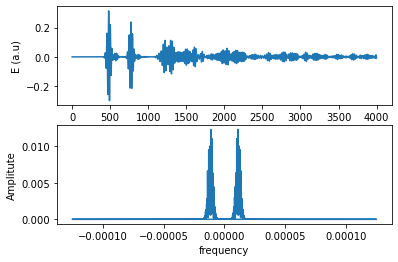
\includegraphics[width=\columnwidth]{202306181.png}}
    \caption{Data plot of Ez and FFT}
    \label{figure_2} 
\end{figure}
\begin{figure}[h]
    \centerline{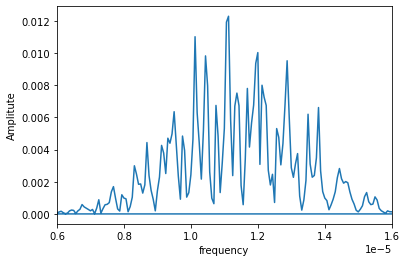
\includegraphics[width=\columnwidth]{202306182.png}}
    \caption{positive side of peak}
    \label{figure_3} 
\end{figure}
\begin{figure}[h]
    \centerline{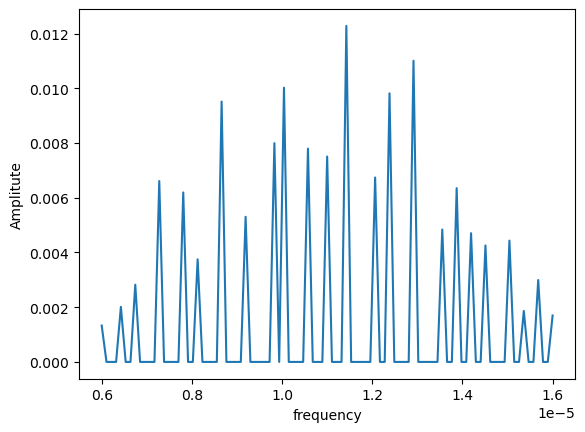
\includegraphics[width=\columnwidth]{202306183.png}}
    \caption{filtering local maximums only}
    \label{figure_4} 
\end{figure}

\end{document}